\documentclass{article}

\usepackage{fancyhdr}
\usepackage{amsmath}
\allowdisplaybreaks
\usepackage{amsthm}
\usepackage{amsfonts}
\usepackage{amssymb}
\usepackage{tikz}
\usepackage[plain]{algorithm}
\usepackage{algpseudocode}
\usepackage{enumitem}
\usepackage{pgfplots}
\pgfplotsset{compat=1.18}
\usepgfplotslibrary{groupplots}
\usepackage{comment}

\usetikzlibrary{automata,positioning,arrows.meta,calc,patterns,fillbetween}

%
% Basic Document Settings
%

\topmargin=-0.45in
\evensidemargin=0in
\oddsidemargin=0in
\textwidth=6.5in
\textheight=9.0in
\headsep=0.25in

\linespread{1.1}

\pagestyle{fancy}
\lhead{\hmwkAuthorName}
\chead{}
\rhead{\hmwkHeaderTitle}
\cfoot{\thepage}

\renewcommand\headrulewidth{0.4pt}
\renewcommand\footrulewidth{0pt}

\setlength\parindent{0pt}

%
% Homework Details
%

\newcommand{\hmwkTitle}{Homework 6}
\newcommand{\hmwkDueDate}{Monday, March 23, 2026}
\newcommand{\hmwkClass}{ICMA 216 Calculus IIIA}
\newcommand{\hmwkClassTime}{Section 1}
\newcommand{\hmwkClassInstructor}{Ruth J. Skulkhu}
\newcommand{\hmwkAuthorName}{\textbf{Jiraroj Wiruchpongsanon (6781617)}}
\newcommand{\hmwkHeaderTitle}{ICMA 216 Calculus IIIA: Homework 6}

%
% Title Page
%

\title{
    \vspace{2in}
    \textmd{\textbf{\hmwkClass:\ \hmwkTitle}}\\
    \normalsize\vspace{0.1in}\small{Due\ on\ \hmwkDueDate}\\
    \vspace{0.1in}\large{\textit{\hmwkClassInstructor\ \hmwkClassTime}}
    \vspace{3in}
}

\author{\hmwkAuthorName}
\date{}

\renewcommand{\part}[1]{\textbf{\large Part \Alph{partCounter}}\stepcounter{partCounter}\\}

%
% Helper Commands
%

\newcounter{partCounter}
\newcommand{\solution}{\textbf{\large Solution}}

\newtheorem*{theorem}{Theorem}

\theoremstyle{remark}
\newtheorem*{remark}{Remark}

\begin{document}

\maketitle
\newpage

\section*{Problem 1 (13.1 Functions of Two Variables)}
Find the domain and range of the function
\begin{enumerate}[label=(\alph*)]
    \item $f(x, y) = x^2 e^{-\sqrt{y+1}}$
    \item $f(x, y) = \sqrt{y - x}\cdot \ln (x + y)$
\end{enumerate}

\medskip
\solution

\begin{enumerate}[label=(\alph*)]
    \item for $\sqrt{y+1}$ to be defined, $y+1 \ge 0 \to y \ge -1$, so 

    \[
    \boxed{D_f \in \{(x,y)\in \mathbb{R}^2 : y \ge -1\}}
    \]

    and for the range, as $x^2 \ge 0$ and $e^{-\sqrt{y+1}} > 0$ and the function can grow infinitely with $x$

    therefore 

    \[
    \boxed{R_f \in [0,\infty)}
    \]

    \medskip
    \begin{center}
    \rule{0.3\linewidth}{0.2pt}
    \end{center}
    \medskip


    \item for $\sqrt{y-x}$ to be defined, $y-x \ge 0$ \hfill (1)

    and for $\ln(x+y)$ to be defined, $x+y > 0$ \hfill (2)

    so \[
    \boxed{D_f \in \{(x,y)\in \mathbb{R}^2 : y-x \ge 0,\ x+y > 0\}}
    \]

    \begin{center}
    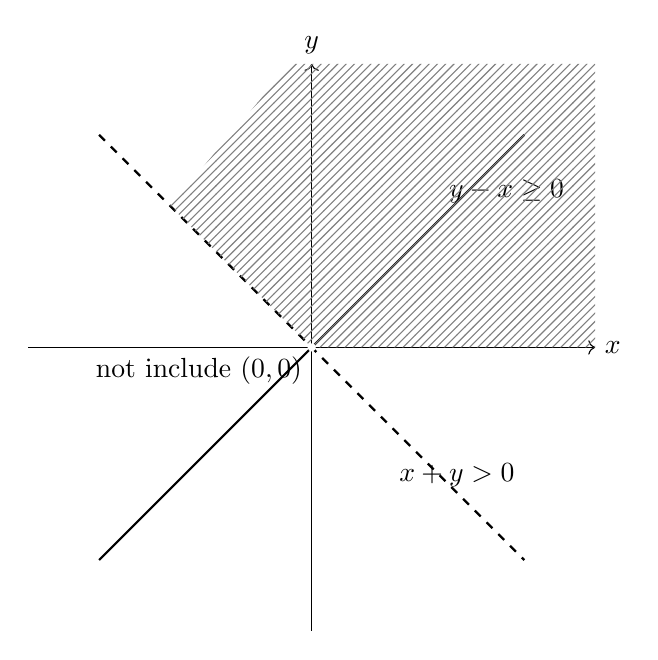
\begin{tikzpicture}[scale=0.9]
        \draw[->] (-4,0) -- (4,0) node[right] {$x$};
        \draw[->] (0,-4) -- (0,4) node[above] {$y$};

        \draw[thick] (-3,-3) -- (3,3);
        \draw[thick,dashed] (-3,3) -- (3,-3);

        \node[anchor=west] at (1.8,2.2) {$y-x \ge 0$};
        \node[anchor=west] at (1.1,-1.8) {$x+y>0$};

        \begin{scope}
            \clip (-4,-4) rectangle (4,4);
            \fill[pattern=north east lines, pattern color=gray]
                (0,0) -- (-2,2) -- (-0.3,4) -- (4,4) -- (4,0) -- cycle;
        \end{scope}

        \filldraw[white] (0,0) circle (1.4pt);
        \node[anchor=north east] at (0,0) {not include $(0,0)$};
    \end{tikzpicture}
    \end{center}

    the graph of domain pair would be looking like this, and as $\sqrt{y-x} \ge 0$ and $\ln(x+y) > 0$

    in case of $\sqrt{y-x} = 0$, this gives the lowest range, and as this function can grow infinitely with $y$, when $x=0$

    therefore \[
    \boxed{R_f \in [0,\infty)}
    \]
\end{enumerate}

\vspace{1em}
\hrulefill

\section*{Problem 2 (13.1 Functions of Two Variables)}
Sketch the graph of the function
\begin{enumerate}[label=(\alph*)]
    \item $f(x, y) = \sqrt{x^2 + y^2 - 1}$
    \item $f(x, y) = 3 - x^2 - y^2$
\end{enumerate}

\medskip
\solution

\begin{enumerate}[label=(\alph*)]
    \item for $\sqrt{x^2+y^2-1}$ to be defined, rearrange as
    \[
    x^2+y^2-1 \ge 0 ;\ f(x,y)\ge 0
    \]
    \[
    x^2+y^2 \ge 1 ;\ f(x,y)\ge 0
    \]

    so \[
    x^2+y^2 = f^2(x,y)+1
    \]

    at $f(x,y)=0 : x^2+y^2=1$

    at $f(x,y)=1 : x^2+y^2=2$

    so \[
    \boxed{D_f \in \{(x,y)\in \mathbb{R}^2 : x^2+y^2 \ge 1\}}
    \]
    \[
    \boxed{R_f \in [0,\infty)}
    \]

    \begin{center}
    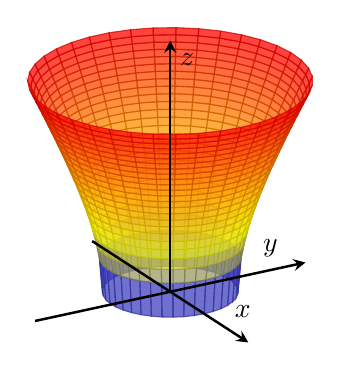
\begin{tikzpicture}
        \begin{axis}[
            width=7cm,
            height=6.8cm,
            view={60}{25},
            axis lines=center,
            axis line style={line width=0.9pt},
            axis on top,
            ticks=none,
            xlabel={$x$}, ylabel={$y$}, zlabel={$z$},
            xmin=-2.3, xmax=2.3,
            ymin=-2.3, ymax=2.3,
            zmin=0, zmax=2.2,
        ]
            \addplot3[
                surf,
                opacity=0.75,
                domain=0:360,
                y domain=1:2.1,
                samples=40,
                samples y=25
            ]
            ({y*cos(x)},{y*sin(x)},{sqrt(y^2-1)});
        \end{axis}
    \end{tikzpicture}
    \end{center}

    \medskip
    \begin{center}
    \rule{0.3\linewidth}{0.2pt}
    \end{center}
    \medskip

    \item rearrange as
    \[
    f(x,y)+x^2+y^2=3
    \]

    at $f(x,y)=3 : x^2+y^2=0$, so the range of $f(x,y)$ is 

    \[
    \boxed{R_f \in (-\infty,3]}
    \]

    and \[
    \boxed{D_f \in \{(x,y)\in \mathbb{R}^2 : x^2+y^2 \ge 0\}}
    \]

    at $f(x,y)=0 : x^2+y^2=3$

    at $f(x,y)=-1 : x^2+y^2=4$

    \begin{center}
    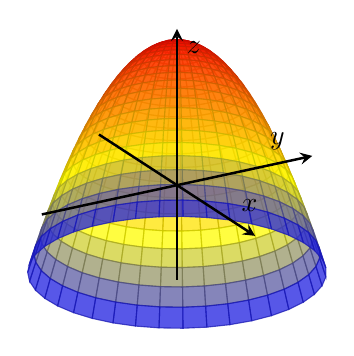
\begin{tikzpicture}
        \begin{axis}[
            width=7cm,
            height=6.8cm,
            view={60}{25},
            axis lines=center,
            axis line style={line width=0.9pt},
            axis on top,
            ticks=none,
            xlabel={$x$}, ylabel={$y$}, zlabel={$z$},
            xmin=-2.3, xmax=2.3,
            ymin=-2.3, ymax=2.3,
            zmin=-2, zmax=3.3,
        ]
            \addplot3[
                surf,
                opacity=0.75,
                domain=0:360,
                y domain=0:2.2,
                samples=40,
                samples y=25
            ]
            ({y*cos(x)},{y*sin(x)},{3-y^2});
        \end{axis}
    \end{tikzpicture}
    \end{center}
\end{enumerate}

\vspace{1em}
\hrulefill

\section*{Problem 3 (13.2 Limits and Continuity)}
Find the limit, if it exists, or show that the limits does not exist.
\begin{enumerate}[label=(\alph*)]
    \item $\lim\limits_{(x,y)\to(3\pi,2\pi)} xy\cos(x-2y)$
    \item $\lim\limits_{(x,y)\to(0,0)} \dfrac{x^4-16y^4}{x^2-4y^2}$
    \item $\lim\limits_{(x,y)\to(0,0)} \dfrac{x^2+y^2}{\sqrt{x^2+y^2+1}-1}$
\end{enumerate}

\medskip
\solution

\begin{enumerate}[label=(\alph*)]
    \item all components supposed to be continuous, so, just substitute $(x,y) = (3\pi,2\pi)$ as
    
    \[
    (3\pi)(2\pi)\cos(3\pi - 2(2\pi))
    \]
    \[
    = 6\pi^2\cos(-\pi)
    \]
    \[
    = \boxed{-6\pi^2}
    \]

    \vspace{1em}

    \medskip
    \begin{center}
    \rule{0.3\linewidth}{0.2pt}
    \end{center}
    \medskip

    \item
    \[
    \lim_{(x,y)\to(0,0)} \frac{x^4-16y^4}{x^2-4y^2}
    = \lim_{(x,y)\to(0,0)} \frac{(x^2+4y^2)(x^2-4y^2)}{(x^2-4y^2)}
    \]
    \[
    = \lim_{(x,y)\to(0,0)} x^2+4y^2
    = 0 + 4(0)
    = \boxed{0}
    \]

    \medskip
    \begin{center}
    \rule{0.3\linewidth}{0.2pt}
    \end{center}
    \medskip

    \item
    \[
    \lim_{(x,y)\to(0,0)} \frac{x^2+y^2}{\sqrt{x^2+y^2+1}-1}
    \]

    use polar substitution:
    \[
    x=r\cos\theta,\quad y=r\sin\theta
    \]

    therefore
    \[
    x^2+y^2=r^2\cos^2\theta+r^2\sin^2\theta
    \]
    \[
    = r^2(\cos^2\theta+\sin^2\theta)
    \]
    \[
    = r^2
    \]

    so, in our case:
    \[
    \lim_{(x,y)\to(0,0)} \frac{x^2+y^2}{\sqrt{(x^2+y^2)+1}-1}
    = \lim_{r\to 0} \frac{r^2}{\sqrt{r^2+1}-1}
    \]
    \[
    = \lim_{r\to 0}\frac{r^2}{\sqrt{r^2+1}-1}\cdot \frac{\sqrt{r^2+1}+1}{\sqrt{r^2+1}+1}
    = \lim_{r\to 0}\frac{r^2(\sqrt{r^2+1}+1)}{r^2+1-1}
    \]
    \[
    = \lim_{r\to 0}\frac{r^2(\sqrt{r^2+1}+1)}{r^2}
    = \lim_{r\to 0}(\sqrt{r^2+1}+1)
    \]
    \[
    = \sqrt{1}+1=\boxed{2}
    \]
\end{enumerate}

\vspace{1em}
\hrulefill

\section*{Problem 4 (13.2 Limits and Continuity)}
Determine the set of points at which the function is continuous.
\begin{enumerate}[label=(\alph*)]
    \item $f(x, y) = \ln (x^2 + y^2 - 4)$
    \item $f(x, y) = \dfrac{\cos(xy)}{e^x-y^2}$
\end{enumerate}

\medskip
\solution

\begin{enumerate}[label=(\alph*)]
    \item for $\ln(x^2+y^2-4)$ to defined, $x^2+y^2-4>0$

    or $x^2+y^2>4$, so
    \[
    \boxed{\{(x,y)\in \mathbb{R}^2 : x^2+y^2>4\}}
    \]

    \begin{center}
    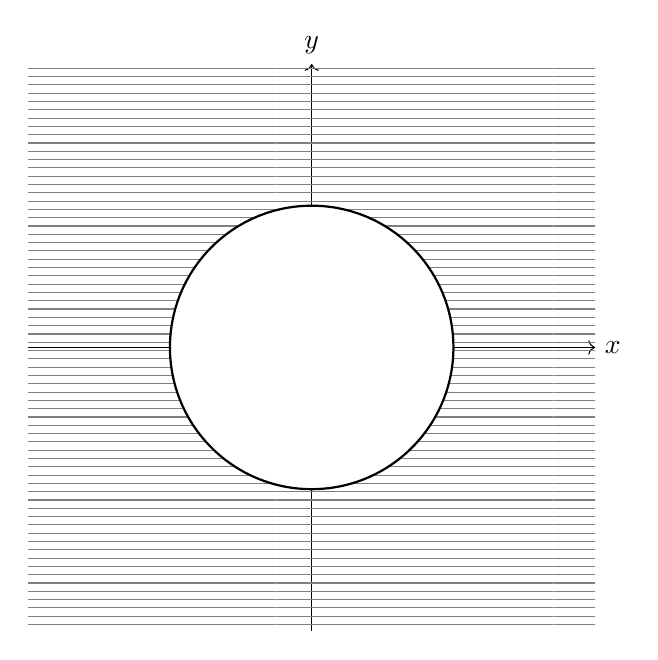
\begin{tikzpicture}[scale=0.9]
        \draw[->] (-4,0) -- (4,0) node[right] {$x$};
        \draw[->] (0,-4) -- (0,4) node[above] {$y$};

        \begin{scope}
            \clip (-4,-4) rectangle (4,4);
            \fill[pattern=horizontal lines, pattern color=gray] (-4,-4) rectangle (4,4);
            \fill[white] (0,0) circle (2);
            \draw[thick] (0,0) circle (2);
        \end{scope}
    \end{tikzpicture}
    \end{center}

    \medskip
    \begin{center}
    \rule{0.3\linewidth}{0.2pt}
    \end{center}
    \medskip

    \item
    \[
    f(x,y)=\frac{\cos(xy)}{e^x-y^2}
    \]

    $\cos(xy)$ is continuous already, so we focus on the denominator

    \[
    e^x-y^2 \ne 0
    \]

    so \[
    \boxed{\{(x,y)\in \mathbb{R}^2 : e^x-y^2 \ne 0\}}
    \]
\end{enumerate}

\end{document}
